\documentclass[mathNotesPreamble]{subfiles}
\begin{document}
%\relscale{1.4} %TODO
\section{13.1: Vectors and the Geometry of Space}
  \begin{defn*}
    \begin{itemize}
      \item \textbf{Vectors}
      
        \begin{minipage}{0.72\linewidth}
          \begin{tasks}[label=\textbullet](1)
          \task Have a \href{https://www.youtube.com/watch?v=bOIe0DIMbI8}{direction and magnitude},
          \task vector $\overrightharp{PQ}$ has a \textit{tail} at $P$ and a \textit{head} at $Q$,
          \task Can be denoted as $\mathbf{u}$ or $\overrightharp{u}$,
          \task Equal vectors have the same direction and magnitude \newline (not necessarily the same position)
        \end{tasks}
        \end{minipage}%
        \begin{minipage}{0.28\linewidth}
          \begin{flushright}
            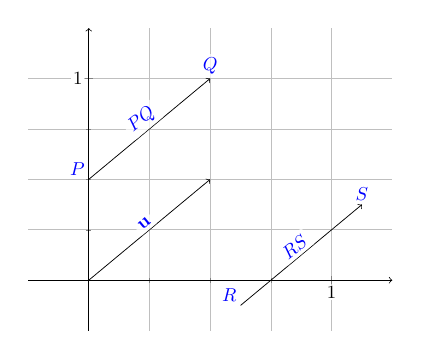
\begin{tikzpicture}[scale=0.675]
              \begin{axis}[
                grid=both, %major,minor
                grid style={line width=0.35pt, draw=gray!50},
                axis lines=center,
                axis line style={black,->},
                xmin=-0.25, xmax=1.25,
                ymin=-0.25, ymax=1.25,
                xtick={0,1},
                ytick={0,1},
                minor x tick num=3,
                minor y tick num=3,
                ticklabel style={font=\normalsize,inner sep=1pt,fill=white,opacity=1.0, text opacity=1},
                every axis plot/.append style={line width=0.95pt, color=blue, samples=100},
                ]
                \draw[->, every node/.style={blue, fill=white, inner sep=2pt, 
                  opacity=0.75, text opacity=1}]
                  (axis cs: 0,0) -- (axis cs: 0.5,0.5) 
                  node[above, sloped, pos=0.5] {$\mathbf{u}$};
                \draw[->, every node/.style={blue, fill=white, inner sep=2pt, 
                  opacity=0.75, text opacity=1}]
                  (axis cs: 0.625,-0.125) -- (axis cs: 1.125,0.375)
                  node[above left, pos=0] {$R$} 
                  node[above, sloped, pos=0.5] {$\overrightharp{RS}$}
                  node[above, pos=1.0] {$S$};
                \draw[->, every node/.style={blue, fill=white, inner sep=2pt, 
                  opacity=0.75, text opacity=1}]
                  (axis cs: 0,0.5) -- (axis cs: 0.5, 1.0)
                  node[above left, pos=0] {$P$} 
                  node[above, sloped, pos=0.5] {$\overrightharp{PQ}$}
                  node[above, pos=1.0] {$Q$};
              \end{axis}
            \end{tikzpicture}
          \end{flushright}
        \end{minipage}
        
      \item \textbf{Scalars} are quantities with magnitude but no direction \newline (e.g. mass, temperature, price, time, etc.)
      \item \textbf{Zero vector}, denoted $\bfO$ or $\overrightharp{0}$, has length $0$ and no direction
    \end{itemize}
  \end{defn*}
  \vspace*{\stretch{1}}

  \textbf{Scalar-vector multiplication:}
    \begin{tasks}[label=\textbullet](1)
      \task Denoted $c\mathbf{v}$ or $c\overrightharp{v}$,
      \task length of vector multiplied by $\abs{c}$,
      \task $c\mathbf v$ has the same direction as $\mathbf v$ if $c>0$, and has the opposite direction as $\mathbf v$ if $c<0$,\newline
            (what if $c=0$?)
      \task $\vecu$ and $\vecv$ are \textbf{parallel} if $\vecu=c\vecv$.\newline
            (what vectors are parallel to $\bfO$?)
    \end{tasks}

  \pagebreak  
  \textbf{Vector Addition and Subtraction:}\newline
  Given two vectors $\vecu$ and $\vecv$, their sum, $\vecu+\vecv$, can be represented by the parallelogram (triangle) rule: place the tail of $\vecv$ at the head of $\vecu$
    \begin{center}
      \begin{tikzpicture}[scale=1.325]
        \coordinate (O) at (0,0);
        \coordinate (A) at (0.125,1.5);
        \coordinate (B) at (2.5,0.375);

        \draw[ClemsonOrange, ->] (O) -- (A) node[pos=0.5, left] {$\vecv$};
        \draw[ClemsonOrange, dashed, ->] ($(O)+(B)$) -- ($(A)+(B)$);
        \draw[ClemsonPurple, ->] (O) -- (B) node[pos=0.5, below] {$\vecu$};
        \draw[ClemsonPurple, dashed, ->] ($(O)+(A)$) -- ($(B)+(A)$);
        \draw[black, ->] (O) -- ($(A)+(B)$) node[pos=0.5, sloped, above] {$\vecu+\vecv$};
      \end{tikzpicture}
    \end{center}
    \vspace*{\stretch{1}}

    The difference, denoted $\vecu-\vecv$, is the sum of $\vecu+(-\vecv)$:
    \begin{center}
      \hspace*{\stretch{1}}
      \begin{tikzpicture}[scale=1.325]
        \coordinate (O) at (0,0);
        \coordinate (A) at (0.125,1.5);
        \coordinate (B) at (2.5,0.375);

        \draw[ClemsonOrange, ->] (O) -- (A) node[pos=0.5, left] {$\vecv$};
        \draw[ClemsonPurple, ->] (O) -- (B) node[pos=0.5, above] {$\vecu$};
        \draw[ClemsonOrange, dashed, <-] ($(B)$) -- ($(B)-(A)$)  
          node[pos=0.5, right] {$\vecv$};
        \draw[black, ->] (O) -- ($(B)-(A)$) 
          node[pos=0.5, sloped, below] {$\vecu-\vecv$};
      \end{tikzpicture}%
      \hspace*{\stretch{1}}%
      \begin{tikzpicture}[scale=1.325]
        \coordinate (O) at (0,0);
        \coordinate (A) at (0.125,1.5);
        \coordinate (B) at (2.5,0.375);

        \draw[ClemsonOrange, ->] (O) -- (A) node[pos=0.5, left] {$\vecv$};
        \draw[ClemsonPurple, ->] (O) -- (B) node[pos=0.5, above] {$\vecu$};
        \draw[ClemsonOrange, dashed, ->] ($(B)$) -- ($(B)-(A)$) 
          node[pos=0.5, right] {$-\vecv$};
        \draw[black, ->] (O) -- ($(B)-(A)$) 
          node[pos=0.5, sloped, below] {$\vecu-\vecv$};
      \end{tikzpicture}
      \hspace*{\stretch{1}}
    \end{center}
    \vspace*{\stretch{1}}
    
  \textbf{Vector Components:}\newline
  A vector $\vecv$ whose tail is at the origin $(0,0)$ and head is at $(v_1,v_2)$ is a \textbf{position vector} (in \textbf{standard position}) and is denoted $\bracket{v_1,v_2}$. The real numbers $v_1$ and $v_2$ are the $x$- and $y$-components of $\vecv$.
    
    \begin{center}
      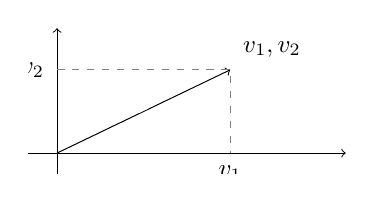
\begin{tikzpicture}[scale=0.9]
        \begin{axis}[
          axis lines=center,
          axis line style={black,->},
          xmin=-0.125, xmax=1.25,
          ymin=-0.125, ymax=0.75,
          xmajorticks=false,
          ymajorticks=false,
          ticklabel style={font=\normalsize,inner sep=1pt,fill=white,opacity=1.0, text opacity=1},
          every axis plot/.append style={line width=0.95pt, color=blue, samples=100},
          width=0.5\linewidth, height=0.3\linewidth
          ]
          \draw[->] (axis cs: 0,0) -- (axis cs: 0.75,0.5) 
            node[above, sloped, pos=0.5, blue, fill=white, inner sep=2pt,
            opacity=0.75, text opacity=1] {$\vecv$};
          \draw[dashed, black!50, every node/.style={black, fill=white, inner sep=5pt,
            opacity=0.75, text opacity=1}] 
            (axis cs: 0,0.5) node[left] {$v_2$} -- 
            (axis cs: 0.75,0.5) node[above right] {$\parens{v_1,v_2}$} -- 
            (0.75,0) node[below] {$v_1$};
        \end{axis}
      \end{tikzpicture}
    \end{center}
    
  Vectors $\vecu=\bracket{u_1,u_2}$ and $\vecv=\bracket{v_1,v_2}$ are equal if and only if $u_1=v_1$ and $u_2=v_2$.
  \pagebreak
  
  \textbf{Magnitude:}\newline
  Given points $P(x_1,y_1)$ and $Q(x_2,y_2)$, the \textbf{magnitude}, or \textbf{length}, of vector\newline $\overrightharp{PQ}=\bracket{x_2-x_1,y_2-y_1}$, denoted $\abs{\overrightharp{PQ}}$, is the distance between points $P$ and $Q$.
    \[\abs{\overrightharp{PQ}}=\sqrt{\parens{x_2-x_1}^2+\parens{y_2-y_1}^2}\]
  
  The magnitude of position vector $\vecv=\bracket{v_1,v_2}$ is $\abs{\vecv}$.
  
  (How do $\abs{\overrightharp{PQ}}$ and $\abs{\overrightharp{QP}}$ relate to each other?)
  
  \begin{center}
    \begin{tikzpicture}[scale=1.0]
      \begin{axis}[
        axis lines=center,
        axis line style={black,->},
        xmin=-0.125, xmax=3.5,
        ymin=-0.125, ymax=1,
        xmajorticks=false,
        ymajorticks=false,
        ticklabel style={font=\normalsize,inner sep=1pt,fill=white,opacity=1.0, text opacity=1},
        every axis plot/.append style={line width=0.95pt, color=blue, samples=100},
        ]
        \coordinate (O) at (axis cs: 0,0);
        \coordinate (A) at (axis cs: 0.75,0.5);
        \coordinate (P) at (axis cs: 1.75, 0.175);
        \coordinate (Q) at ($(P)+(A)$);
        \draw[->] (O) -- (A) 
          node[above, pos=1, blue, fill=white, inner sep=2pt,
          opacity=0.75, text opacity=1] {$\vecv=\bracket{v_1,v_2}$};
        \draw[->] (P) node[left] {$P(x_1,y_1)$} -- (Q) node[above] {$Q(x_2,y_2)$};
        \draw[dashed] (Q) |- (P) 
          node[right, pos=0.25] {$y_2-y_1$}
          node[below, pos=0.75] {$x_2-x_1$};
      \end{axis}
    \end{tikzpicture}
    
  \fbox{\parbox{0.9875\linewidth}{
    \underline{Note:} The norm, denoted $\norm[\vecu]$ or $\norm[\vecu]_2$, is equivalent to the magnitude of a vector.
  }}
  \end{center}
  \vspace*{\stretch{1}}
  
  \textbf{Equation of a Circle:}
    \begin{defn*}
      A \textbf{circle} centered at $(a,b)$ with radius $r$ is the set of points satisfying the equation
        \[\parens{x-a}^2+\parens{y-b}^2=r^2.\]
      A \textbf{disk} centered at $(a,b)$ with radius $r$ is the set of points satisfying the inequality
        \[\parens{x-a}^2+\parens{y-b}^2\leq r^2.\]
    \end{defn*}
  \pagebreak
  
  \textbf{Vector Operations in Terms of Components}
  \begin{defn*}[Vector Operations in $\bbr^2$]
    Suppose $c$ is a scalar, $\vecu=\bracket{u_1,u_2}$, and $\vecv=\bracket{v_1,v_2}$.
      \begin{alignat*}{2}
        \vecu+\vecv&=\bracket{u_1+v_1,u_2+v_2}&\hspace*{25pt}& \textnormal{\textcolor{blue}{ Vector addition}}\\
        \vecu-\vecv&=\bracket{u_1-v_1,u_2-v_2}&& \textnormal{\textcolor{blue}{ Vector subtraction}}\\
        c\vecu&=\bracket{cu_1,cu_2}&& \textnormal{\textcolor{blue}{ Scalar multiplication}}
      \end{alignat*}
  \end{defn*}
  %TODO show |cu|=|c|*|u|
  \begin{center}
    \begin{tikzpicture}[scale=0.825]
      \begin{groupplot}[
        group style={group size=3 by 1, horizontal sep=1cm, vertical sep=2cm},
        axis lines=center,
        axis line style={black,->},
        ticklabel style={font=\normalsize,inner sep=0.5pt,
          fill=white,opacity=1.0, text opacity=1},
        every axis plot/.append style={line width=0.95pt, color=blue, samples=100}
        ]
        \nextgroupplot[
          xmin=-0.5, xmax=3.35,
          ymin=-0.25, ymax=2,
          xtick={0.75,2,2+0.75},
          ytick={0.375,1.5,1.5+0.375},
          xticklabels={$v_1$, $u_1$, $u_1+v_1$},
          yticklabels={$u_2$,$v_2$,$u_2+v_2$}
          ]
          \coordinate (O) at (0,0);
          \coordinate (A) at (0.75,1.5);
          \coordinate (B) at (2.0,0.375);
          \coordinate (AB) at ($(A)+(B)-(O)$);

          \draw[ClemsonOrange, ->, line width=1.5pt] (O) -- (A) node[pos=0.7, left] {$\vecv$};
          \draw[ClemsonOrange, dashed, ->] (B) -- (AB);
          \draw[ClemsonPurple, ->, line width=1.5pt] (O) -- (B) node[pos=0.65, above] {$\vecu$};
          \draw[ClemsonPurple, dashed, ->] (A) -- (AB);
          \draw[black, ->] (O) -- (AB) node[pos=0.5, sloped, above] {$\vecu+\vecv$};
          \draw[dashed, black!50] (O|-AB) --(AB)--(AB|-O);

        \nextgroupplot[
          xmin=-0.125, xmax=1.5,
          ymin=-0.25, ymax=2,
          xtick={0.75,1.5*0.75},
          ytick={1,1.5*1},
          xticklabels={$u_1$, $c u_1$},
          yticklabels={$u_2$, $c u_2$}
          ]
          \coordinate (O) at (0,0);
          \coordinate (A) at ($(0.75,1)$);
          \coordinate (cA) at ($1.5*($(A)-(O)$)+(O)$);

          \draw[black, ->] (O) -- (cA) node[pos=0.75, sloped, above] {$c\vecu$};
          \draw[ClemsonOrange, ->, line width=1.5pt] (O) -- (A) node[pos=0.5, below] {$\vecu$};
          \draw[dashed, black!50] (O|-cA) --(cA)--(cA|-O);

        \nextgroupplot[
          xmin=-0.75, xmax=1.0,
          ymin=-1, ymax=1.5,
          xtick={0.75,-0.75*0.75},
          ytick={1,-0.75*1},
          xticklabels={$u_1$, $c u_1$},
          yticklabels={$u_2$, $c u_2$}
          ]
          \coordinate (O) at (0,0);
          \coordinate (A) at ($(0.75,1)$);
          \coordinate (cA) at ($-0.75*($(A)-(O)$)+(O)$);

          \draw[ClemsonOrange, ->, line width=1.5pt] (O) -- (A) node[pos=0.5, below] {$\vecu$};
          \draw[black, ->] (O) -- (cA) node[pos=0.5, sloped, above] {$c\vecu$};
          \draw[dashed, black!50] (O|-cA) --(cA)--(cA|-O);
      \end{groupplot}
    \end{tikzpicture}
  \end{center}
  \begin{ex*}
    Let $\vecu=\bracket{1,2}$, $\vecv=\bracket{-2,3}$, $c=2$, and $d=3$. Find the following:
    \begin{tasks}[after-item-skip=10pt, label=](2)
      \task $\vecu+\vecv$
      \task $c\vecu$
      \task $c\vecu+d\vecv$
      \task $\vecu-c\vecv$
    \end{tasks}
  \end{ex*}

  \begin{defn*}
    A \textbf{unit vector} is any vector with length 1.
    
    In $\bbr^2$, the \textbf{coordinate unit vectors} are $\bfi=\bracket{1,0}$ and $\bfj=\bracket{0,1}$.
  \end{defn*}
  \begin{ex*}
    Let $\vecu=\bracket{-7,3}$. Find two unit vectors parallel to $\vecu$. Find another vector parallel to $\vecu$ with a magnitude of $2$.
  \end{ex*}
  \vspace*{\stretch{1}}
  \pagebreak
  
  \noindent
  \fbox{\parbox{0.9875\linewidth}{
    \textbf{Properties of Vector Operations:}
    
    Suppose $\vecu$, $\vecv$, and $\bm{w}$ are vectors and $a$ and $c$ are scalars. Then the following properties hold (for vectors in any number of dimensions).
    \begin{quote}
      \TabPositions{0.4\linewidth}
      \begin{enumerate}
        \item 
          $\vecu+\vecv=\vecv+\vecu$
          \tab \textcolor{blue}{Commutative property of addition}
        \item 
          $\parens{\vecu+\vecv}+\bm w=\vecu+\parens{\vecv+\bm w}$
          \tab \textcolor{blue}{Associative property of addition}
        \item 
          $\vecv+\bfO=\vecv$
          \tab \textcolor{blue}{Additive identity}
        \item 
          $\vecv+\parens{-\vecv}=\bfO$
          \tab \textcolor{blue}{Additive inverse}
        \item 
          $c\parens{\vecu+\vecv}=c\vecu+c\vecv$
          \tab \textcolor{blue}{Distributive property 1}
        \item 
          $\parens{a+c}\vecv=a\vecv+c\vecv$
          \tab \textcolor{blue}{Distributive property 2}
        \item 
          $0\vecv=\bfO$
          \tab \textcolor{blue}{Multiplication by zero scalar}
        \item 
          $c\bfO=\bfO$
          \tab \textcolor{blue}{Multiplication by zero vector}
        \item 
          $1\vecv=\vecv$
          \tab \textcolor{blue}{Multiplicative identity}
        \item 
          $a\parens{c\vecv}=\parens{ac}\vecv$ 
          \tab \textcolor{blue}{Associative property of scalar multiplication}
      \end{enumerate}
    \end{quote}
  }}

  \pagebreak
\end{document}
